\documentclass[a4paper, 14pt]{extarticle}	% general format

%%%% Charset
\usepackage{cmap}							% make PDF files searchable and copyable
\usepackage[utf8x]{inputenc}				% accept different input encodings
\usepackage[T2A]{fontenc}					% russian font
\usepackage[russian]{babel}					% multilingual support (T2A)

%%%% Graphics
\usepackage[dvipsnames]{xcolor}			% driver-independent color extensions
\usepackage{graphicx}						% enhanced support for graphics
\usepackage{wrapfig}						% produces figures which text can flow around

%%%% Math
\usepackage{amsmath}						% American Mathematical Society (AMS) math facilities
\usepackage{amsfonts}						% fonts from the AMS
\usepackage{amssymb}						% additional math symbols

%%%% Typograpy (don't forget about cm-super)
\usepackage{microtype}						% subliminal refinements towards typographical perfection
\linespread{1.3}							% line spacing
\usepackage[left=2.5cm, right=1.5cm, top=2.5cm, bottom=2.5cm]{geometry}
\setlength{\parindent}{0pt}					% we don't want any paragraph indentation
\usepackage{parskip}						% some distance between paragraphs

%%%% Tables
\usepackage{tabularx}						% tables with variable width columns
\usepackage{multirow}						% for tabularx
\usepackage{hhline}							% for tabularx

%%%% Graph
\usepackage{tikz}							% package for creating graphics programmatically
\usetikzlibrary{arrows}						% edges for tikz

%%%% Other
\usepackage{url}							% verbatim with URL-sensitive line breaks
\usepackage{fancyvrb}						% sophisticated verbatim text (with box)
%------------------------------------------------------------------------------

\begin{document}

%------------------------------------------------
\begin{titlepage}
\thispagestyle{empty}

\begin{center}
Санкт-Петербургский политехнический университет Петра Великого\\
Институт Информационных Технологий и Управления \\*
Кафедра компьютерных систем и программных технологий \\*
\hrulefill
\end{center}

\vspace{10em}

\begin{center}
\Large Отчёт по самостоятельно работе\\по предмету «Теория распознавания образов» \\
\end{center}

\vspace{1em}

% \linebreak
\begin{center}
\textsc{\textbf{Локализация и отслеживние лиц на изображении}}
\end{center}

\vspace{16em}

\begin{flushleft}
Работу выполнил студент гр. 53501/3 \hrulefill Мартынов С. А. \\
\vspace{1.5em}
Работу принял преподаватель \hrulefill Никитин К. В. \\
\end{flushleft}

\vspace{\fill}

\begin{center}
Санкт-Петербург \\
2015
\end{center}

\end{titlepage}
%------------------------------------------------
\setcounter{page}{2}
\tableofcontents

%------------------------------------------------------------------------------

\newpage
\section*{Введение}
\addcontentsline{toc}{section}{Введение}

Локализация человеческого лица с последующей идентификацией давно находится в списке наиболее важных задач для исследователей в области систем машинного зрения и искусственного интеллекта. Множество исследований, проводимых ведущими научными центрами, так и не позволило создать универсальную систему компьютерного зрения, способную к локализации и распознаванию лица человека при различных условиях.

Причиной тому явилось сразу множество факторов, среди которых:
\begin{itemize}
\item высокая вариативностью лиц, обусловленной анатомическими особенностями людей;
\item различный уровень освещенности объектов, зависящих от типа, количества и характеристик направленности источников света;
\item необходимость обнаружения лиц, имеющих различное пространственное положение.
\end{itemize}

Зачастую особенности системы, использующей локализацию и распознавание лиц может накладывать дополнительные ограничения на скорость работы (близкой к реальному времени), аппаратным ресурсам (процессор, объём памяти) и экономичности (аккумулятора).

Кроме скоростных характеристик, от алгоритма требуется обеспечение малого (порядка 5\%) количества ложных распознаваний. В системах, реализующих существующие методы распознавания, при увеличении уровня распознаваний свыше 90\% наблюдается существенный рост числа ложных решений, что затрудняет их практическое использование. Прежде чем распознавать лицо, необходимо убедиться в его присутствии на изображении. Для чего применяются известные методы обнаружения и распознавания лиц на изображениях (метод главных компонент, нейронные сети, метод опорных векторов). Результативность применения метода определяется спецификой решаемой задачи. Поэтому построение метода распознавания лиц, обеспечивающего высокий уровень достоверности решения при отсутствии ограничений на исходные изображения, является весьма актуальной задачей.

Целью данной работы является обзор основных методов обнаружения лиц (под обнаружением лиц на изображении будем понимать процесс локализации областей изображения, содержащих лица людей; границы искомых областей в в общем случае размыты, однако чаще всего подразумевается минимальный описывающий прямоугольник), обеспечивающих повышение достоверности распознавания объектов анализа, снижение уровня ложных распознаваний, уменьшение времени обучения классификатора и времени предварительной обработки изображения.

%------------------------------------------------------------------------------

\newpage
\section{Признаки изображений}

Вычисление признаков изображения является одиним из важнейших аспектов при распознавании визуальных образов. Признак в данном контексте это произвольные дескрипторы изображения, полученные в результате обработки исходных данных. Качество детектирования определяется информативностью выделенных признаков, а вычислительная сложность алгоритмов выделения -- скоростю работы системы распознавания. В самом простом случае, признаком может являться яркость или цвета пикселей, составляющих исследуемое изображение.

Имеется множество различных примеров классификации признаков по типу, но обычно выделяют три основные категории:
\begin{itemize}
\item яркостные -- базируются на перепадах яркости в пикселях;
\item текстурные -- описываются с помощью повторяющихся базовых элементов текстур;
\item геометрические -- описывают фрагменты фигур и контуров, присутствующих на изображении.
\end{itemize}

Тип вычисляемых признаков определяется содержимым изображения, которое надо описать. Обобщенное человеческое лицо, как графический паттерн, из-за своей сложности может быть описано сразу всеми типами признаков. 

\subsection{Признаки Хаара}

Вейвлеты Хаара -- это семейство базисных функций, открытое в начале XX века Альфредом Хааром. Вейвлеты Хаара ортогональны, обладают компактным носителем, хорошо локализованы в пространстве, являются кусочно-постоянными функциями с разрывами 1-го рода. Из-за своей простой и быстрой формулы расчета они повсеместно применяются в задачах анализа нестационарных сигналов.


Рассмотрим множество кусочно-постоянных функций, определенных наинтервале $[0, 1)$, состоящем из $2^l$ подинтервалов равной длины. Пусть функции, определенные на всем единичном интервале, образуют пространство $V^0$; кусочнопостоянные функции, одна часть каждой из которых определена на интервале $[0, \frac{1}{2})$, а другая на $[\frac{1}{2}, 1)$ образуют пространство $V^1$ и т.д. Таким образом, пространство $V^l$ содержит все кусочно-постоянные функции, определенные на всех $2^l$ подинтервалах единичного интервала. Базис Хаара представляет собой множество функций, определенных для каждого пространства $V^l$ . Базисные функции называются масштабирующими функциями и порождаются сдвигами и растяжениями прямоугольного импульса.

\begin{gather}
\varphi(x) =
  \begin{cases}
    1,\qquad 0\le x \le 1,\\
    0,\qquad otherwise.
 \end{cases}
\end{gather}

\begin{gather}
\varphi_{l,t}(x) = 2^{1/2}\varphi(2^lx-t)
\end{gather} 

Масштаб определяется множителем $2^{l/2}$, а сдвиг задается параметром $t = 0 \ldots{} 2^{l-1} - 1$. Интеграл от масштабирующей функции на интервале $[-\infty, +\infty]$ равен единице. Соответствующий набор вейвлет-функций Хаара, ортогональный масштабирующим функциям, определяется посредством смещения и растяжения своего материнского вейвлета.

\begin{gather}
\psi(x) =
  \begin{cases}
    1,\qquad 0\le x \le \dfrac{1}{2},\\
    -1,\qquad \dfrac{1}{2}\le x \le 1,\\
    0,\qquad otherwise.
 \end{cases}
\end{gather}

\begin{gather}
\psi_{l,t}(x) = 2^{1/2}\psi(2^lx-t)
\end{gather} 

Интеграл от вейвлет-функции на интервале $[-\infty, +\infty]$ принимает нулевое значение.

Одномерный базис Хаара, заданный в $V^2$, может быть распространен на плоскость двумя способами. Стандартная композиция получается, когда одномерное вейвлет-преобразование применяется для каждого измерения поочередно: новым базисом служат всевозможные тензорные произведения функций $\psi_{l,t}(\bullet)$. Нестандартный базис выводится путем смещений и растяжений двумерной масштабирующей функции (5) и трех двумерных материнских вейвлетов.

\begin{gather}
\varphi(x,y)=\varphi(x)\varphi(y)
\end{gather}

\begin{gather}
\psi^m(x,y) =
  \begin{cases}
    \psi(x)\varphi(y),\qquad m=1,\\
    \varphi(x)\psi(y),\qquad m=2,\\
    \psi(x)\psi(y),\qquad m=3.
 \end{cases}
\end{gather}

Такой подход имеет преимущества перед стандартной композицией, поскольку обеспечивает лучшее пространственное разрешение за счет некоторой избыточности базиса (рис. 1). При одномерном преобразовании расстояние между соседними вейвлетами $\psi_{l,t}(x)$ составляет $2^l$, в стандартном двумерном базисе -- $2^{l-1}$, а в нестандартном -- $2^{l-2}$.

\begin{figure}[h!]
\centering
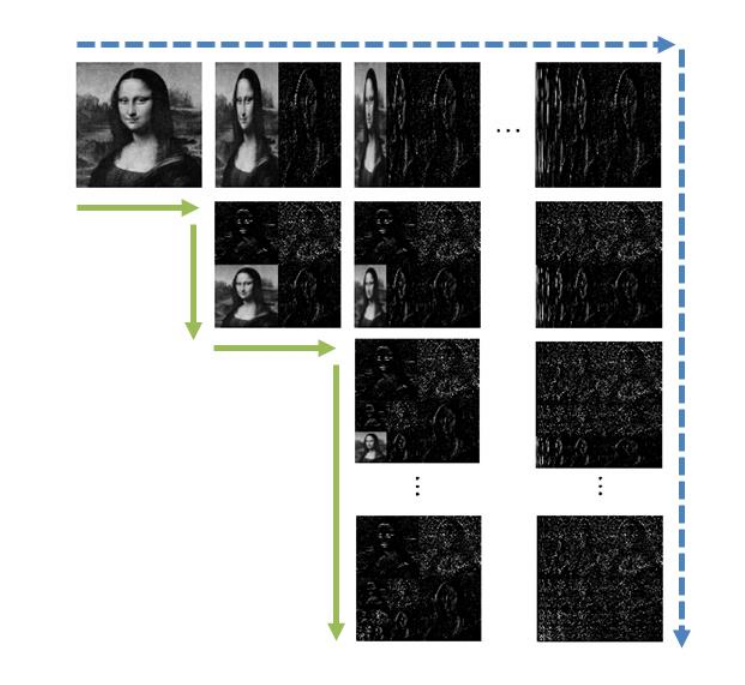
\includegraphics[scale=0.6]{res/pic001}
\caption{Пример вейвлет-декомпозиции двумя способами: стандартным (пунктирная стрелка) и нестандартным (сплошная стрелка)}
\end{figure}

На рис. 2 схематично представлены материнские вейвлеты, полученные по формуле (6). Темная область соответствует отрицательным значениям вейвлета, светлая -- положительным.

\begin{figure}[h!]
\centering
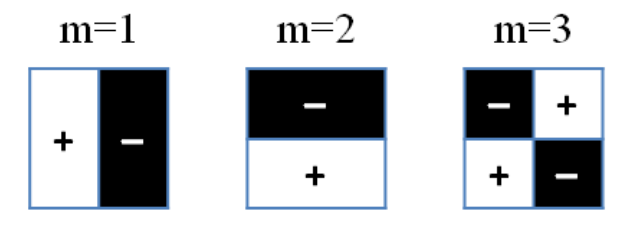
\includegraphics[scale=0.6]{res/pic002}
\caption{Три двумерных материнских вейвлета}
\end{figure}

Признаки Хаара -- признаки цифрового изображения, вычисляемые с помощью функций, схожих по своей структуре с двумерными вейвлетами Хаара. Специалистами было предложено использовать материнские вейвлеты Хаара в качестве ядер для свертки исходного изображения. Каждый вычисляемый признак $H$ представлен комбинацией прямоугольников $h_i$. При подсчете признака окно $h$ скользит по изображению, и вычисляется среднее значение пикселей, покрываемых каждым прямоугольником -- $\mu(i)$ . Прямоугольникам соответствуют веса $w_i \in \{−1, +1\}$, определяющие с каким знаком войдет среднее значение пикселей в общую сумму. Согласно свойству интеграла от масштабирующих функций, веса удовлетворяют условию нулевой суммы:

\begin{gather}
\sum\limits_{k=1}^N w_i=0
\end{gather}

Выражение для вычисления признака имеет следующий вид:

\begin{gather}
H = \sum\limits_{k=1}^N w_i \mu_i
\end{gather}

На рисунке 3 изображены примеры расширенных признаков Хаара, предложенных Виолой и Джонсом (верхний ряд) и Ленхард [18] (нижний ряд).

\begin{figure}[h!]
\centering
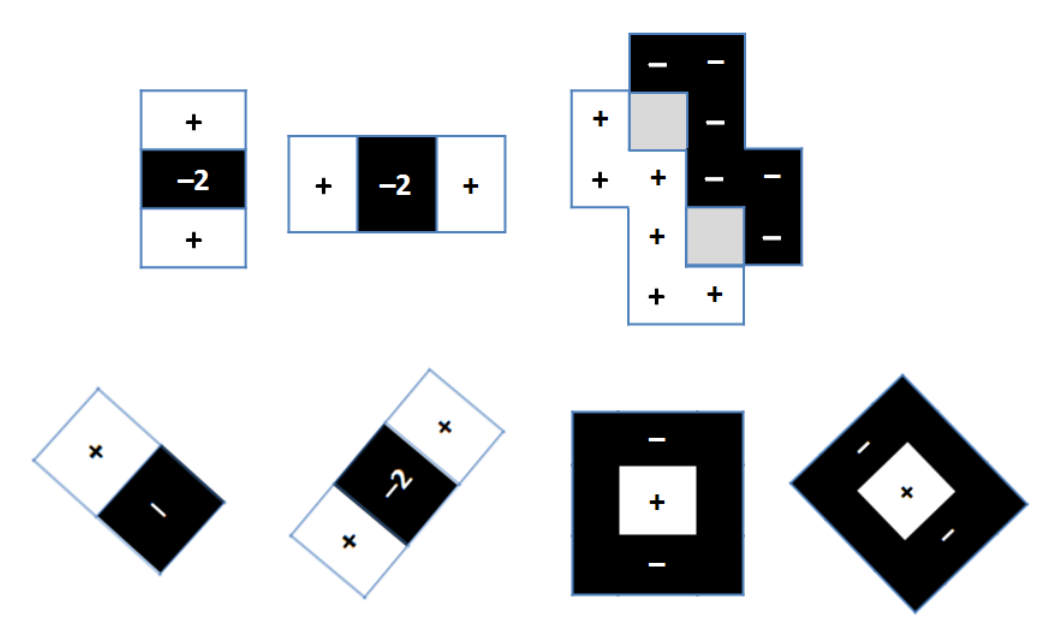
\includegraphics[scale=0.45]{res/pic003}
\caption{Расширенный набор признаков Хаара}
\end{figure}

В пользу признаков Хаара говорит наличие для них эффективных вычислительных схем. Виола и Джонс предлагают использовать интегральное изображение для ускорения процедуры подсчета признаков. Интегральное изображение $\overline{\overline{I}}$ это матрица той же размерности, что и исходное изображение $I$, элементы которой определяются следующим образом:

\begin{gather}
\overline{I}(x,y) = \sum\limits_{\substack{x' \le x\\y' \le y}} I(x',y')
\end{gather}

Тогда среднее значение $\mu_i$ для прямоугольника $h_i$ с вершинами в точках $A_i$ , $B_i$ , $C_i$ , $D_i$ с площадью $S_i$ (рис 1) может быть посчитано за четыре арифметические операций над пикселями интегрального изображения:

\begin{gather}
\mu_i = (\overline{I}(A_i) + \overline{I}(B_i) - \overline{I}(C_i) - \overline{I}(D_i)) / S_i
\end{gather}

Для признаков Ленхард, повернутых на $45\,^{\circ}$, также существует быстрая схема вычислений. Для этого используется понятие таблицы суммированных областей, аналогичное определению интегрального изображения, выраженного формулой (9). Для вычисления таких признаков Ленхард вводится понятие таблицы суммированных областей, которые повернуты на угол, вычисляемой по следующей формуле:

\begin{gather}
\overline{\overline{I}}(x,y) = \sum\limits_{\substack{x' \le x\\x' \le x - |y' - y|}} I(x',y')
\end{gather}

Среднее значение $\mu_i$ для прямоугольника $h_i$ с вершинами в точках $A_i$ , $B_i$ , $C_i$ , $D_i$ с площадью $S_i$ и углом поворота $\alpha_i = 45\,^{\circ}$ может быть также вычислено по формуле (10) для $\overline{I} = \overline{\overline{I}}$.

\subsection{Локальные бинарные шаблоны}

Порядковое измерение контраста (ordinal contrast measure) является порождением простого концепта: относительное важнее абсолютного. При анализе различных изображений мы можем отмечать значительные изменения абсолютных величин: цветов, яркости, текстурных элементов. Однако, взаимные порядковые отношения между соседними величинами, отражающие структуру изображенных объектов, подвержены меньшим изменениям. Порядковое кодирование контраста (ordinal contrast encoding) используется для вычисления существенных контрастных различий (contrast polarity) между двумя пикселями или регионами изображений. Оператор ставит в соответствие паре пикселей 1, если первый пиксель ярче второго или 0, в противном случае. Такой код удобен для вычислений, а информационная энтропия измерений максимальна, поскольку для случайных паттернов практически равновероятны значения 0 и 1.

Операция   порядкового   кодирования   контраста $T \equiv T(X)$ обладает  следующими свойствами инвариантности:

\begin{gather}
T(X) \equiv T(X+a) \equiv T(X \times a) \equiv T(X^a), \\
a \equiv const > 0 \nonumber
\end{gather}

Census-преобразование (рис. 4) проецирует локальное окружение заданного  пикселя  в  битовую  строку.  Полученная  битовая  строка  может быть использована  в  качестве  дескриптора  области  изображения. Обозначим  через $(x_c, y_c)$ координаты  центрального  пикселя, $(x_p, y_p)$ -- координаты  смежного пикселя, $f(\bullet)$ -- значение яркости пикселя в точке с заданными координатами. Тогда census-преобразование может быть представлено следующим образом:

\begin{gather}
T(X) = \otimes_{p=0}^{p-1}s(f(x_p, y_p)-f(x_c, y_c))
\end{gather}

\begin{gather}
s(x) =
  \begin{cases}
    1,\qquad x < 0,\\
    0,\qquad x \ge 0.
 \end{cases}
\end{gather}

\begin{figure}[h!]
\centering
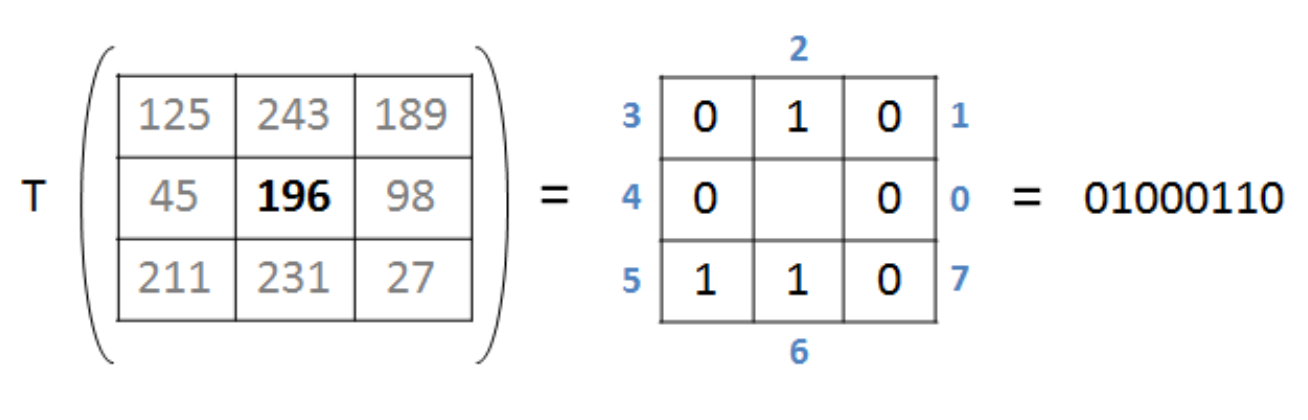
\includegraphics[scale=0.35]{res/pic004}
\caption{Census-преобразование}
\end{figure}

В качестве метрики схожести между census-образами пикселей изображений, используется расстояние Хэмминга, то есть рассчитывается число различающихся битов  в  соответствующих  битовых строках.  Основное  ограничение census-преобразования  в  том,  что  оно  охватывает малый  регион  анализируемого изображения вблизи центрального пикселя -- этого может оказаться недостаточно для выделения ключевых текстурных характеристик.

Обобщенный случай census-преобразования -- метод локальных бинарных шаблонов (ЛБШ), который был предложен Пиетикайненым. Количество соседних  точек,  участвующих  в  построении  дескриптора,  и  их  удаленность  от центрального пикселя определяются параметрами P и R соответственно:

\begin{gather}
LBP_{P,R}(x_c, y_c) =  \sum\limits_{p=0}^{P-1}s(f(x_p, y_p)-f(x_c, y_c))2^P
\end{gather}

Каждому  анализируемому  множеству  пикселей  оператор ЛБШ ставит  в соответствие   натуральное   число,   определяющееся   из   равенства (15). Принципиальным отличием ЛБШ от Census-преобразования является то, что ЛБШ-преобразование может применяться к соседним пикселям, лежащим на некоторой окружности  радиуса $R \ge 1$ c центром  в  пикселе $x_c$ (рисунок 5).  Координаты пикселей $x_p$ могут быть рассчитаны исходя из соотношений:

\begin{gather}
s(x) =
  \begin{cases}
    x_p=x_c + R \cos \frac{2 \pi p}{P} \\
    y_p=y_c - R \sin \frac{2 \pi p}{P}
 \end{cases}
\end{gather}

\begin{figure}[h!]
\centering
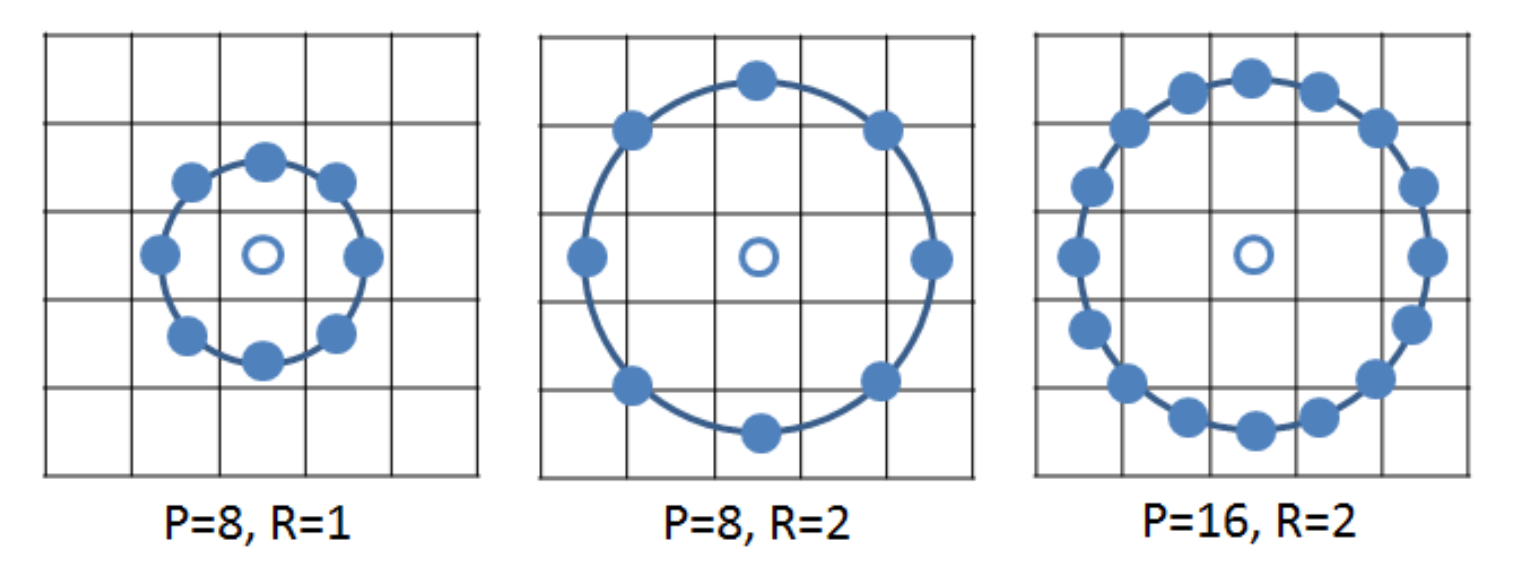
\includegraphics[scale=0.33]{res/pic005}
\caption{LBP-преобразование с различным радиусом и количеством соседе}
\end{figure}

Если  координаты  точки $(x_p, y_p)$ не  соответствуют  центру  какого-либо пикселя изображения, то значение яркости в данной точке может быть получено с помощью интерполяции. Одним из самых простых и распространенных способов является  билинейная  интерполяция.  Если  положить,  что  четыре  ближайших  к $(x_p, y_p)$ пикселя лежат на вершинах единичного квадрата, $x = x_p - | x_p |$, $y = y_p - | y_p |$ , то значение яркости в точке $(x_p, y_p)$ может быть вычислено по значениям пикселей в вершинах квадрата:

\begin{gather}
f(x_p, y_p) \approx 
\begin{bmatrix}
  1-x & x
\end{bmatrix}
\begin{bmatrix}
  f(0,0) & f(0,1)\\
  f(1,0) & f(1,1)
\end{bmatrix}
\begin{bmatrix}
  1-y\\
  y
\end{bmatrix}
\end{gather}

При P=8, R=1 формула ЛБШ принимает классическую форму. Многомасштабный анализ, основанный на ЛБШ, может производиться  двумя способами. В первом случае меняется радиус R оператора ЛБШ-преобразования. Во  втором  случае  уменьшается  размерность  исходного  изображения  с последующим применением ЛБШ-оператора фиксированного радиуса. 
Оператор (15),  строго  говоря,  не  является  инвариантным  к  поворотам исходного изображения. Предлагается проецировать область пикселя в  битовую  строку,  записанную  как  циклический  код.  Случайно  совершая циклические  перестановки,  ищется  совпадение  с  одним  из  наперед  заданных бинарных шаблонов. Оператор $LBD_{P,R}^{ri}$ возвращает номер совпавшего с битовой строкой  бинарного  шаблона.  Для  случая,  когда $P=8$ имеется ряд унифицированных  шаблонов  (uniform patterns), которые 
получаются из циклических сдвигов нескольких категорий битовых строк (рисунок 6): 
\begin{enumerate}
\item Линии (lines): 01111111, 00000001.
\item Углы (corners): 00111111, 00011111, 00001111, 00000011.
\item Край (edge): 00000111.
\end{enumerate}

Перечисленные категории образуют 56 паттернов, к ним добавляется еще два шаблона,  которые  не  варьируются  циклическим  смещением:  11111111 --
плоскость  (flat),  00000000 -- точка  (spot).  Оператор,  использующий  58 унифицированных шаблонов для описания области изображения, обозначается как $LBD_{P,R}^{ri2u}$.

\begin{figure}[h!]
\centering
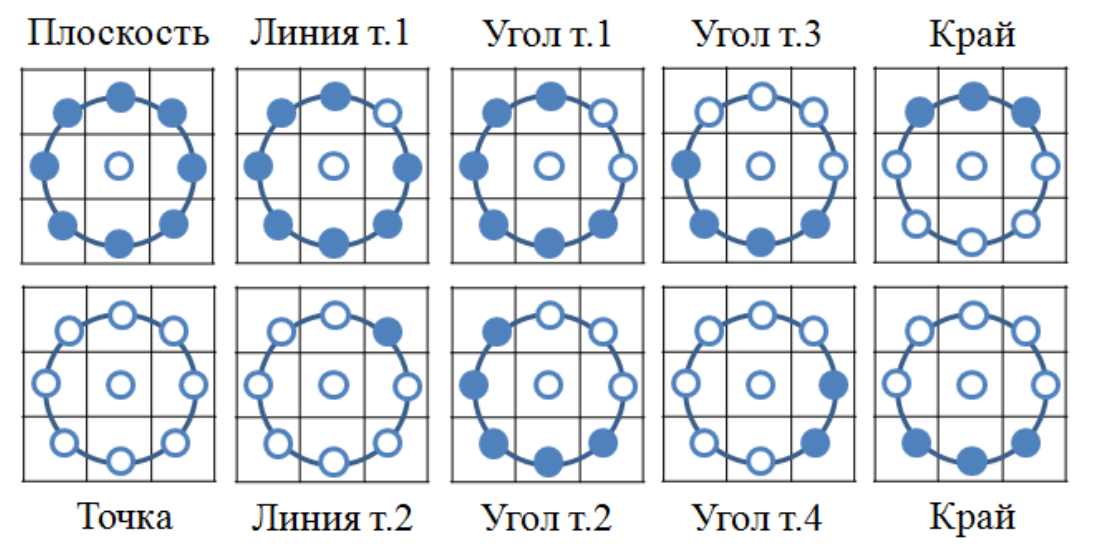
\includegraphics[scale=0.45]{res/pic006}
\caption{Примеры унифицированных шаблонов}
\end{figure}

В качестве дескриптора для анализа изображений используется гистограмма ЛБШ-образов пикселей. Пусть область значений $A$ оператора $LBD_{P,R}^{ri2u}$ разбита на равные промежутки: 
$ A = \cup_i(a_{i-1},a_i]$

\begin{gather}
n_{P,R}(i)=\sum\limits_{j=1}^{N}1_{\{LBD_{P,R}^{ri2u}(x_{c_j},y_{c_j})\in(a_{i-1},a_i]\}}
\end{gather}

$n_{P,R}(i)$ -- число значений, попавших в i-ый интервал. Пусть $N = |A|$. Тогда нормализованная гистограмма ЛБШ-признаков принимает следующий вид:

\begin{gather}
h_{P,R}(i)=\frac{n_{P,R}(i)}{N \times (a_i - a_{i-1})}
\end{gather}

\subsection{Двухмерное косинусное преобразование}

%------------------------------------------------------------------------------

\newpage
\section{Методы бинарной классификации признаков}
%------------------------------------------------------------------------------

\newpage
\section{Нейронные сети}

%------------------------------------------------------------------------------

\newpage
\section*{Заключение}
\addcontentsline{toc}{section}{Заключение}

%------------------------------------------------------------------------------

\newpage
\section*{Список литературы}
\addcontentsline{toc}{section}{Список литературы}


\end{document}